\documentclass[12pt,a4paper]{book}
\usepackage[utf8]{inputenc}												% Codificación
\usepackage[spanish,es-tabla]{babel}									% Lenguaje español, Tabla n: 
\usepackage[T1]{fontenc}												% Agregar fuentes con acentos
\usepackage{amsmath}													% Paquetes necesarios  para matemáticas
\usepackage{amsfonts}
\usepackage{amssymb}
\usepackage{makeidx}													% Paquete para indices
\usepackage{graphicx}													% Para manejar imagenes
\graphicspath{{imagenes/}}												% Ruta de las imagenes, solo escribir nombre de la imagen
\usepackage[top=1in, left=0.9in, right=1.25in, bottom=1in]{geometry}	% Margenes
\author{Emmanuel Javier Tobón Ramírez}
\title{Tesis}
\date{}
%-------------------------------------------------------------------------------
%                            Paquetes adicionales                              %
%-------------------------------------------------------------------------------
\decimalpoint
\usepackage{xcolor}
\usepackage{ragged2e}
\usepackage{etoolbox}

\usepackage{comment}											% Comentarios largos
\usepackage{pdfpages}											% Incluir portada echa en Inkscape
\usepackage{setspace}											% Interlineado
\usepackage{makecell}											% Para tablas
\usepackage{xcolor}												% Colores en tablas
\usepackage{colortbl}
\usepackage{array}												% Necesario para algunas tablas
\usepackage[inline]{enumitem}									% Personalizar itemize
\usepackage{multicol}											% Item 2 columns											% Necesario para algunas tablas
\usepackage{subcaption}											% Subfiguras
%-------------------------------------------------------------------------------
%                            Comandos matematicos                              %
%-------------------------------------------------------------------------------
\usepackage{steinmetz}											% Para representar fasores
\usepackage{bm}													% Bold math  \bm command
\newcommand{\binomb}[2]{\genfrac{[}{]}{0pt}{}{#1}{#2}}


\apptocmd{\frame}{}{\justifying}{} % Allow optional arguments after frame.

\setbeamertemplate{footline}
{
  \leavevmode%
  \hbox{%
  \begin{beamercolorbox}[wd=.333333\paperwidth,ht=2.5ex,dp=1ex,center]{author in head/foot}%
    \usebeamerfont{author in head/foot}Ciro Fabián Bermúdez Márquez
  \end{beamercolorbox}%
  \begin{beamercolorbox}[wd=.333333\paperwidth,ht=2.5ex,dp=1ex,center]{title in head/foot}%
    \usebeamerfont{title in head/foot}Benemérita Universidad Autónoma de Puebla
  \end{beamercolorbox}%
  \begin{beamercolorbox}[wd=.333333\paperwidth,ht=2.5ex,dp=1ex,right]{date in head/foot}%
    \usebeamerfont{date in head/foot}Facultad de Ciencias de la Electrónica\hspace*{2em}
    \insertframenumber{} / \inserttotalframenumber\hspace*{2ex} 
  \end{beamercolorbox}}%
  \vskip0pt%
}


%\usefonttheme{serif}
\usefonttheme[onlymath]{serif}



\setbeamertemplate{caption}[numbered]
\theoremstyle{definition}
	\newtheorem{defn}{Definición}
	\newtheorem{exmp}{Ejemplo}
	\newtheorem{law}{Ley}
	
	
%-------------------------------------------------------------------------------
%                            Libreria de codigos                               %
%-------------------------------------------------------------------------------
% Paquetes necesarios
\usepackage{listings}
\usepackage{xcolor}

% Tipos de letra personalizadas
\def\lstbasicfont{\fontfamily{pcr}\selectfont\scriptsize}
\def\vhdlbasicfont{\fontfamily{cmtt}\selectfont\scriptsize}

% Colores personalizados
\definecolor{codegreen}{rgb}{0,0.6,0}
\definecolor{codepurple}{rgb}{0.58,0,0.82}

\definecolor{codegray}{rgb}{0.5,0.5,0.5}
\definecolor{backcolour}{rgb}{0.95,0.95,0.92}
\definecolor{codeorange}{RGB}{254, 100, 35}

% Deficion de lenguajes perzonalizados

% Definicion de lenguaje MATLAB
\lstdefinelanguage{matlabfloz}{%
  alsoletter={...},%
  morekeywords={%                             % keywords
		break,case,catch,classdef,continue,else,
		elseif,end,for,function,global,if,
		otherwise,parfor,persistent,
		return,spmd,switch,try,while,...},        % Use the matlab "iskeyword" command to get those
  comment=[l]\%,                              % comments
  morecomment=[l]...,                         % comments
  morecomment=[s]{\%\{}{\%\}},                % block comments
  morestring=[m]'                             % strings 
}[keywords,comments,strings]%

% Estilos MATLAB
\lstdefinestyle{MATLAB}{
	frame=single,
	rulecolor=\color{black},
	framexleftmargin=4mm,
	xleftmargin=2mm,
	language=matlabfloz,
  commentstyle=\color{codegreen},
  keywordstyle=\color{blue}, %magenta
  numberstyle=\tiny\color{black},
  stringstyle=\color{codepurple},
  basicstyle=\lstbasicfont\tiny,
  breakatwhitespace=false,         
  breaklines=true,                 
  captionpos=b,                    
  keepspaces=true,                 
  numbers=left,                    
  numbersep=5pt,                  
  showspaces=false,                
  showstringspaces=false,
  showtabs=false,                  
  tabsize=2    
}

% Estilos MATLAB en codigo
\lstdefinestyle{MATLAB_preview}{
%	frame=single,
%	rulecolor=\color{black},
%	framexleftmargin=4mm,
%	xleftmargin=2mm,
	language=matlabfloz,
    commentstyle=\color{codegreen},
    keywordstyle=\color{blue}, %magenta
%    numberstyle=\tiny\color{black},
    stringstyle=\color{codepurple},
    basicstyle=\lstbasicfont\small,
    breakatwhitespace=false,         
    breaklines=true,                 
    captionpos=b,                    
    keepspaces=true,                 
%    numbers=left,                    
%    numbersep=5pt,                  
    showspaces=false,                
    showstringspaces=false,
    showtabs=false,                  
    tabsize=2    
}

\renewcommand{\lstlistingname}{Código}% Listing -> Algorithm
\renewcommand{\lstlistlistingname}{Lista de códigos}% 
%-------------------------------------------------------------------------------
%                             Archivos a incluir                               %
%-------------------------------------------------------------------------------
\includeonly{
%	portada,
%	agradecimientos,
%	resumen,
%	ch1,
	ch2
%	ch3,
%	ch4,
%	ch5,
%	Ap_A,
%	Ap_D
}
%-------------------------------------------------------------------------------
%-------------------------------------------------------------------------------
\begin{document}

\frontmatter
%\includepdf[pages=-]{portada.pdf}

%\layout

%% ----------------------------------------------------------

\begin{titlepage}

\noindent
%\hspace{0cm}						% Ajustar centrado
\setlength{\unitlength}{1pt}
\begin{picture}(\x,\y)(0,0)

%% Lineas guia, hay que comentarlas al terminar
	% Margenes
%	\linethickness{2mm}
%	\put(0,0){\line(1,0){\x}}
%	\put(0,0){\line(0,1){\y}}
%	\put(\x,\y){\line(0,-1){\y}}
%	\put(\x,\y){\line(-1,0){\x}}
%
%	% Cuadricula
%	\linethickness{0.3mm}
%	\multiput(0, 0)(0,\cuadro){30}{\line(1, 0){\x}}		
%	\multiput(0, 0)(\cuadro, 0){20}{\line(0, 1){\y}}
%	
%	% Linea central de guia
%	\linethickness{1.5mm}
%	\setlength{\unitlength}{\cuadro pt}
%	\put(12,0){\line(0,1){30}}				
	
%% Logos				
	\setlength{\unitlength}{\cuadro pt}				% Unidad de un cuadro
	\put(0,25){
\includegraphics[width= \fpeval{\cuadro *5}pt ]{logo_buap.eps}}	
	\put(0.7,2.8){
\includegraphics[width= \fpeval{\cuadro *3.8}pt]{logo_fce.eps}}
	
%% Formula para centrar
% 5 + [ 7 - (Cant de cuadros de palabra)/2 ]
% Ejemplo: Facultad de Ciencias la Electrónica 		ocupa 9.5 cuadros
% 			5 + [ 7 - 4.75] = 7.25
	
%% Texto de Universidad, Facultad y nombre de Tesis
	\put(4.9,29){\begin{large}\textsc{Benemérita Universidad Autónoma de Puebla}\end{large}}
	\put(6.2,27){\begin{large}\textsc{Facultad de Ciencias la Electrónica}\end{large}}
	\put(9.6,25){\begin{large}\textsc{Título de tesis}\end{large}}
	\put(7,23){\begin{large}\textsc{Antenas flexibles multibanda}\end{large}}
%	\put(5.2,22.1){\begin{large}\textsc{usando hardware analógico reprogramable}\end{large}}
%	\put(5.8,21.2){\begin{large}\textsc{y su aplicación en un oscilador caótico}\end{large}}
	
%% Letras TESIS
	\put(6.9,18){\begin{Huge}
	\textsc{T} \hspace{\cuadro pt} 
	\textsc{E} \hspace{\cuadro pt} 
	\textsc{S} \hspace{\cuadro pt} 
	\textsc{I} \hspace{\cuadro pt} 
	\textsc{S}
	\end{Huge}}
	
%% Carrera, Nombre, Asesores, Lugar y fecha
	\put(7.15,16.5){\begin{large}\textsc{que para obtener el título de:}\end{large}}
	\put(9,15.5){\begin{large}\textsc{Lic. en Electrónica}\end{large}}
	\put(10.5,14.5){\begin{large}\textsc{presenta:}\end{large}}
	\put(6.95,13.5){\begin{large}\textsc{Emmanuel Javier Tobón Ramírez}\end{large}}
	\put(10.6,10){\begin{large}\textsc{Asesores:}\end{large}}
	\put(6.7,9){\begin{large}\textsc{Dr. Richard  Torrealba Melendez}\end{large}}
	\put(8.7,7){\begin{large}\textsc{Puebla, Puebla, 2020}\end{large}}
	
%% Lineas decorativas
	\linethickness{0.7mm}
	\put(5,28.5){\line(1,0){14}}			% Horizontal grande
	\put(2.5,9.5){\line(0,1){15}}			% Vertical grande
	\linethickness{0.3mm}
	\put(5,28.2){\line(1,0){14}}			% Horizontal
	\put(2.8,9.5){\line(0,1){15}}			% Vertical pequeña der
	\put(2.2,9.5){\line(0,1){15}}			% Vertical pequeña izq
\end{picture}
\end{titlepage}
	\thispagestyle{empty}												% Limpiar estilos de pagina


\onehalfspacing															% Desde este punto interlineado de 1.5
% 	\spacing{1.213}
	\chapter{Agradecimientos}

Agradezco a mi familia por el apoyo incondicional que siempre me han dado, es debido a ellos que estoy cumpliendo esta meta.

Agradezco especialmente a mi madre Juana Márquez Huerta por siempre haber estado presente cuando la necesité.

Agradezco inmensamente a mi novia Julisa Verdejo Palacios porque es debido a ella que comencé con este trabajo.

Agradezco a mi asesor de tesis, el Dr. Jesús Manuel Muñoz Pacheco por su paciencia, confianza, apoyo y conocimientos compartidos.

Agradezco al CONACYT que a través del programa Ciencia Básica me otorgó una beca para el desarrollo de esta tesis de licenciatura mediante el proyecto no. 258880 de nombre SÍNTESIS DE INTEGRADORES DE ORDEN FRACCIONARIO USANDO HARDWARE ANALÓGICO REPROGRAMABLE Y SU APLICACIÓN EN UN OSCILADOR CAÓTICO.

Agradezco a la Facultad de Ciencias de la Electrónica de la BUAP, a mis profesores y compañeros por ayudarme en cada paso de esta travesía.



\pagestyle{normalstyle}													% Estilos de pagina personalizados
\tableofcontents            											% Genera el índice
\addcontentsline{toc}{chapter}{\contentsname}

\listoffigures              											% Indice de figuras
\listoftables               											% Indice de tablas
\lstlistoflistings

	\chapter{Resumen}


	En este trabajo de tesis se presenta en primera instancia el análisis teórico de la expansión de fracciones continuas (CFE) para su utilización en la creación de integradores de orden fraccionario. Se hace un análisis del error que esta aproximación presenta y se generará una metodología de diseño de acuerdo al orden fraccionario.
	
	Utilizando hardware analógico embebido (FPAA) y por medio del dispositivo NI ELVIS II+ se realizará la implementación física de los integradores de orden fraccionario y se medirá su respuesta en frecuencia. Obtenidos los resultados se obtendrá un análisis comparativo teórico contra experimental y se desarrollaran gráficas de mérito para facilitar el diseño.
	
	Finalmente se utilizarán las metodologias obtenidas para realizar la implementación de un oscilador caótico de orden fraccionario poniendo a prueba así el rendimiento de los integradores.
	\pagestyle{Resumen}	
	
\mainmatter
\pagestyle{normalstyle}	
	\chapter{Introducción}
	
	El caos se refiere a un tipo de comportamiento dinámico complejo que posee algunas características muy especiales, tales como extrema sensibilidad a pequeñas variaciones de la condición inicial, trayectorias encerradas en el espacio de fase pero con un exponente de Lyapunov positivo, un espectro de potencia continuo entre muchas otras. En pocas palabras, el caos es simplemente un comportamiento impredecible de un sistema determinista. Es de interés resaltar que los sistemas caóticos ya eran conocidos desde hace mucho tiempo atrás y que no fue hasta hace poco que se logró demostrar que el caos puede ser controlado y debido a esto impactar en muchas áreas, tanto en áreas cercanas a la electrónica como técnicas de modulación, sistemas de comunicación, técnicas de encriptación de datos, como también en áreas  relacionadas a los sistemas biológicos, reacciones químicas, toma de decisiones críticas en política, economía, eventos militares, etc  \cite{Munoz-Pacheco2010}. El caos es un fenómeno que ocurre en muchos sistemas no lineales, donde la naturaleza determinista de la estructura se conjuga con la irregularidad del comportamiento, esto significa que, a pesar del hecho de que el sistema se describe mediante un conjunto de ecuaciones diferenciales ordinarias, donde todos los términos son perfectamente conocidos, su comportamiento es irregular y muy sensible a las condiciones iniciales. La primera evidencia de imprevisibilidad en los sistemas deterministas se encuentra en el trabajo del matemático y científico Henri Poincaré sobre el movimiento celestial, mientras que la primera formulación del caos en un modelo matemático expresado por un conjunto de ecuaciones diferenciales ordinarias que exhiben el caos se debe al matemático y meteorólogo Edward Lorenz que estaba estudiando un modelo de movimiento del aire en la atmósfera y descubrió cómo pequeñas variaciones en los valores iniciales de las variables de su modelo dieron como resultado predicciones meteorológicas divergentes \cite{Buscarino2014}. Para el momento de esos estudios faltaba una prueba experimental definitiva del caos y la tecnología y poder de cómputo no eran suficientes para pensar aún en soluciones y aún más distantes las aplicaciones. Debido al constante avance de la electrónica, hoy en día somos capaces de sintetizar mediante dispositivos electrónicos sistemas caóticos, utilizando técnicas de modelado e implementación es posible crear representaciones de estos, no obstante, todas estas se basan en aproximaciones que aún no han sido exploradas en su totalidad. 
	Por otro lado el cálculo fraccionario es un tema que tiene más de 300 años de antigüedad y que se remonta a cartas enviadas a Leibniz por parte de Bernoulli y de L'Hôspital preguntando acerca de la derivada a la $1/2$ e indagando sobre su significado. Con el paso de los años la teoría de cálculo fraccionario se fue desarrollando pasando por las manos de nombres conocidos como: Euler, Lagrange, Laplace, Fourier hasta llegar a Liouville, Riemann, Grünwald, Letnikov, Caputo entre muchos otros \cite{Petras2011}. Pero aún con todo ese desarrollo no fue hasta hace poco que la comunidad científica comenzó a interesarse por esta rama del cálculo y la razón principal de este cambio es que los cálculos necesarios para cualquier posible implemetación eran demasiado complejos y lentos, un panorama totalmente diferente se vive en la actualidad, el rápido avance de la tecnología ha logrado realizar avances notables en esta área. El rango de aplicaciones para el cálculo fraccionario es inmenso, por mencionar algunas de las más recientes, la modelación de derivadas fraccionarias para obtener una mejor representación comportamental de un sistema industrial metalúrgico \cite{Petras2019}, la incorporación de dinámica de orden fraccional para mejorar la robustez de un control PI/PID para motores DC \cite{Tepljakov2016,Khubalkar2018}, la modelación de señales biológicas como ECG, EMG y EEG debido a su respuesta de magnitud de 20$\alpha$dB, modelos fisiológicos basados en ecuaciones diferenciales lineales que describen fenómenos complejos en el cuerpo humano como la oxigenación de la sangre entre otros \cite{Ortigueira2011}.
	El cálculo fraccionario y los sistemas caóticos se complementan al añadir un nivel de profundidad en la creación de osciladores caóticos modelados como un conjunto de ecuaciones diferenciales no lineales fraccionarias las cuales son materia prima para la creación de nuevas aplicaciones y áreas de desarrollo. 
	
	\section{Justificación}
	
	Los osciladores caóticos son una área de oportunidad emergente cuyas aplicaciones han aumentado en los ultimamos años, a principios del siglo XX se comenzó a explorar el uso de osciladores caóticos para la detección de señales pequeñas basados en la propiedad  de extrema sensibilidad a pequeños cambios de la condición inicial que estos presentan \cite{Wang1999}, y en la seguridad de sistemas de comunicación ya sea en tiempo continuo o discreto \cite{Tepina2002}.  Casi al mismo tiempo los sistemas de orden fraccionario comenzaron a formar parte del interés de la comunidad científica nuevamente y se abrieron las puertas al control de sistemas de orden fraccionario y como implementarlos \cite{Chen2009,Das2007}. Los intentos de implementaciones físicas de sistemas de orden fraccionario han avanzado mucho recientemente y se pueden categorizar en digitales, los cuales utilizan sistemas discretos basados en microprocesadores o FPGA cuya complejidad radica en poder generar un software robusto que sea lo suficiente fiable \cite{Gunay2017}. Por el otro lado se encuentran las implenetaciones analógicas, las cuales son de gran interés en este trabajo. En la literatura de esta área podemos encontrar implementaciones basadas en la construcción de capacitores electrolíticos especiales que se aproximan al comportamiento fraccionario pero cuya fabricación es compleja \cite{Jesus2008}, métodos electroquímicos que trabajan con compuestos químicos de difícil manipulación y tienen ordenes que no pueden modificarse fácilmente \cite{Biswas2006}, finalmente y en lo que se enfocará este trabajo se encuentran las aproximaciones de funciones racionales en un ancho de banda determinado utilizando los métodos de Newton, Oustaloup, Carlson, Matsuda o expansión de fracciones continuas (CFE) \cite{Charef2006,Krishna2011,Krishna2008}. Una vez que la función de trasferencia es obtenida, esta se sintetiza utilizando diferentes metodologías, como la realización pasiva que hace uso de resistencias, capacitores e inductores, con el inconveniente de poder ajustarse a los valores comerciales, o la realización activa, que utiliza las técnicas de diseño basadas en amplificadores operacionales \cite{Tepljakov2013, Dorcak2012}. Una alternativa a estas metodologías es la sintetización utilizando dispositivos analógicos embebidos programables FPAA (Field Programable Analog Array). Las FPAA han demostrado ser una arquitectura prometedora que facilita mucho el proceso de implemetación de circuitos analógicos debido a que su interfaz se basa en Módulos Analógicos Configurables (CAM), los cuales son bloques que pueden interconectarse fácilmente y representan desde circuitos sencillos como integradores, derivadores, sumadores o inversores hasta circuitos más complejos como filtros completos y multiplicadores \cite{Fragoulis2009}. Sin embargo en el ámbito tanto de integradores fraccionarios como de osciladores caóticos aun existen metodologías nuevas por explorar, en algunos artículos científicos ya se ha mostrado como implementar un integrador de orden fraccionario utilizando la aproximación de Oustaloup y CAMs de filtros bilineales \cite{Caponetto2006}, no obstante la cantidad de recursos para crear un solo integrador es muy grande, lo cual da pie a ser mejorado utilizando aproximaciones diferentes, por ejemplo la expansión de fracciones continuas. De mismo modo implementar osciladores caóticos basados en sistemas de ecuaciones diferenciales de orden entero utilizando una FPAA ya ha sido explorado en años recientes \cite{Li2018}, sin embargo los basados en sistemas de ecuaciones diferenciales de orden fraccionario aun se encuentran en una etapa temprana y son ideales para ser estudiados. Las aplicaciones de los osciladores caóticos van en aumento y ser capaces de implemetarlos se ha vuelto una tarea relevante, estos ahora se están utilizando en aplicaciones médicas, como en la detección de señales cardíacas \cite{Jiang2010} y en la creación de radares UWB que tienen futuro prometedor en la medicina \cite{Kumari2017}.
	
	\section{Objetivos}
	
		\subsection{Objetivo general}
			Diseño e implementación electrónica de integradores de orden fraccionario mediante una expansión de fracciones continuas para su aplicación en sistemas caóticos.		
		
		\subsection{Objetivos específicos}
			\begin{itemize}
			\item Analizar el método de expansión de fracciones continuas para generar una metodología de diseño en MATLAB.
			\item Caracterizar el error de la expansión de fracciones continuas para generar reglas de diseño.
			\item Diseñar e implementar en FPAA el integrador de orden fraccionario con aproximaciones de ordenes superiores.
			\item Diseñar e implementar de FPAA un oscilador caótico de orden fraccionario. 
		\end{itemize}
		
		
%% Para formato de propuesta de tesis
%\begin{comment}
	\section{Descripción}

	Este trabajo se desarrollará haciendo en primer lugar una investigación profunda del método de expansión de fracciones continuas para la creación de integradores de orden fraccionario y un análisis de su estructura matemática para generar algoritmos eficientes que obtengan la función racional aproximada. Una vez obtenidos estos algoritmos se hará un análisis del error de la función racional aproximada con respecto al integrador fraccionario ideal dependiente del orden de la aproximación y el orden fraccionario. Una vez concluidos los análisis teóricos se procederá a realizar la implementación física de los integradores fraccionarios utilizando la tarjeta Quad Apex v2.0 la cual contiene 4 FPAA. Se realizará un análisis de las diferentes metodologías que se pueden seguir en la implementación haciendo mediciones de la respuesta en frecuencia (Diagramas de Bode). Se pretende que estas mediciones den como resultado reglas de diseño que faciliten el proceso de implementación y mejoren en manejo de recursos en la FPAA. Finalmente se implementará físicamente un oscilador caótico basado en un sistema de ecuaciones diferenciales de orden fraccionario.
	
	\newpage
	\section{Diagrama de bloques}	
	\begin{figure}[hbtp]
	\centering
	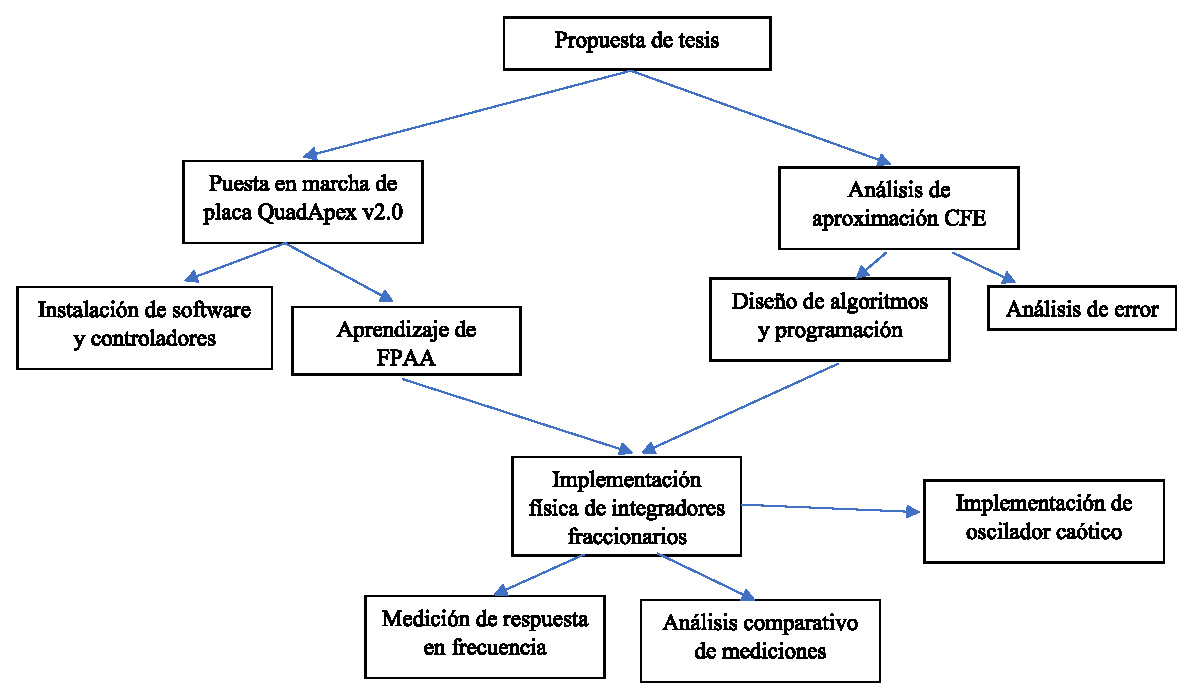
\includegraphics[width = 11cm]{diagrama_de_bloques.eps}
	\caption{Diagrama de bloques}
	\end{figure}
	
	\section{Cronograma de actividades}
	\begin{figure}[hbtp]
	\centering
	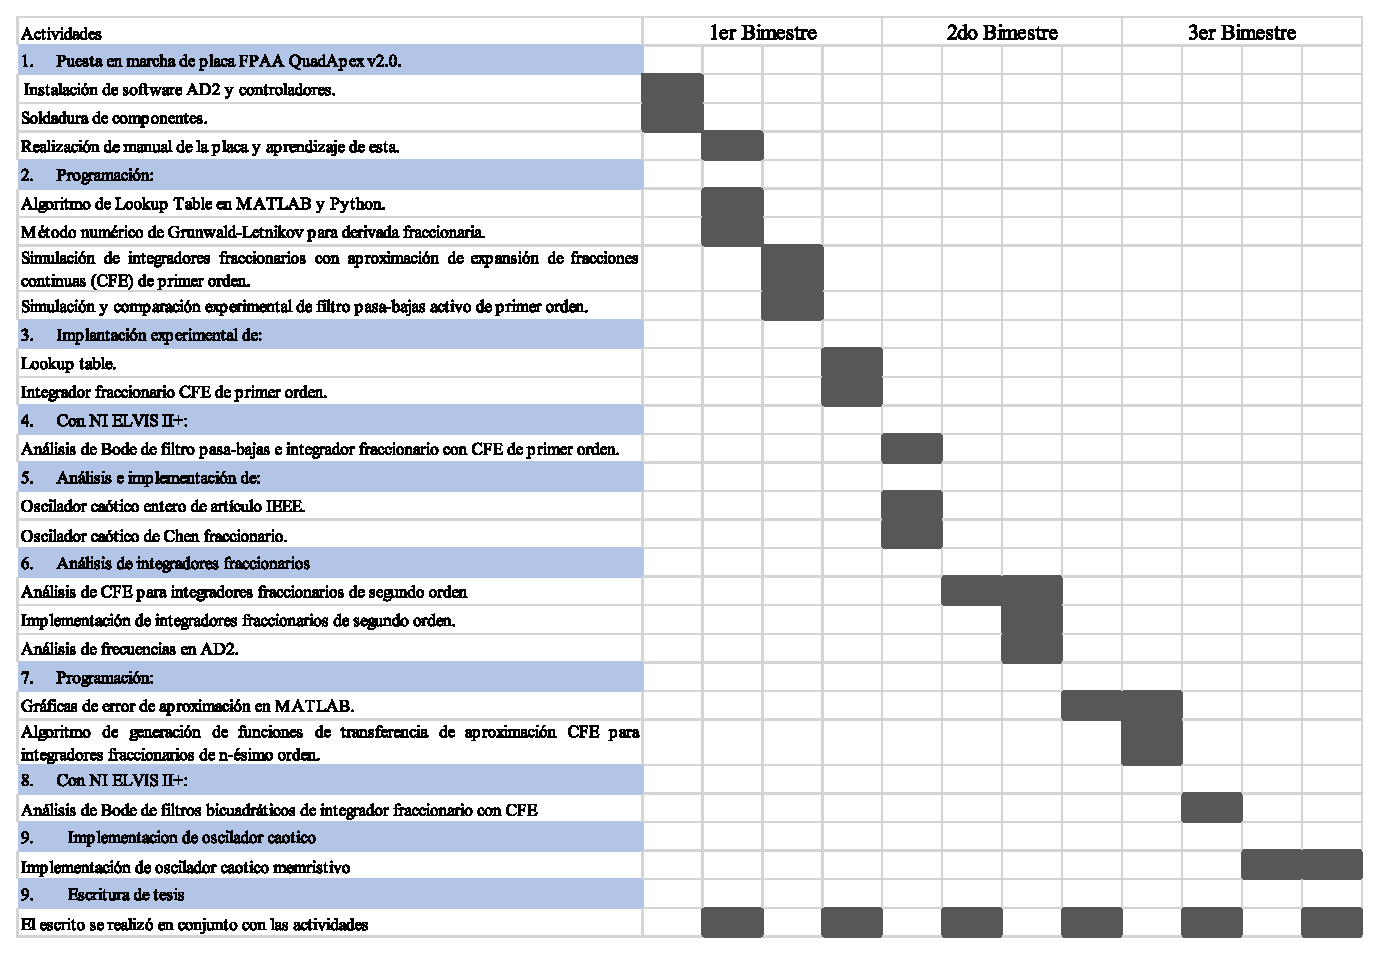
\includegraphics[width = 14.8cm]{cronograma_de_actividades.eps}
	\caption{Cronograma de actividades}
	\end{figure}		
		
%\end{comment}
%		
	
	
	
	
	\chapter{Fundamentos teóricos}		
	Cuando se comienza a estudiar cálculo de orden entero es necesario familiarizarse con la notación de los operadores matemáticos de la derivada y la integral, con el cálculo fraccionario ocurre lo mismo. En la actualidad la notación más utilizada para el cálculo entero es la dada por Leibniz en (1686), donde el operador diferencial de n-ésimo orden esta definido como: $\frac{d^{n}}{dt^{n}}$, $D_{t}^{n}$ o simplemente $D^{n}$ con $n \in \mathbb{N}$. Utilizando el mismo razonamiento, puede definirse su operador inverso (antiderivada) de manera que el operador inverso de la derivada de n-ésimo orden está dado por: $_{a}D^{-n}_{t}$, donde $n \in \mathbb{N}$ y $a \in \mathbb{R}$ representa el límite inferior del dominio de la región donde se aplica dicho operador.
			
	Para generalizar el operador diferencial e integral para orden fraccionario se considera que este puede definirse para parámetros de orden real o incluso complejo. Esto implica que los operadores pueden definirse respectivamente como: $D^{\alpha}$ y $_{a}D^{\alpha}_{t}$ con $ \alpha \in \mathbb{R}$. 
		
	Es importante tener presente que no una hay una única definición para los operadores diferencial e integral fraccional, sino varias expresiones definidas por diferentes autores, entre las mas usadas se encuentran la definición de Grünwald-Letnikov (GL), la de Riemann-Liouville (RL) y la de Caputo (Ca), cada una de estas con sus ventajas y desventajas desde el punto de vista del análisis matemático, complejidad computacional e implementación \cite{Petras2011}.
			
	\section{Definición de Grünwald-Letnikov}
	
		\subsection{Definición de derivada de Grünwald-Letnikov}
			
		\subsection{Definición de integral de Grünwald-Letnikov}

		\subsection{Método numérico para la definición de GL}

	\section{Definición de Riemann-Liouville}

		\subsection{Definición de integral de Riemann-Liouville}
		
		\subsection{Definición de derivada de Riemann-Liouville}
		
	\section{Transformada de Laplace de integrales y derivadas fraccionarias}
	
	\section{Expansión de fracciones continuas (CFE)}\label{sec:CFE}
	
	\subsection{Análisis de error de la CFE}
	                                                                 
	\section{Escalamiento en frecuencia}

	\section{Teoría de filtros}
	
		\subsection{Filtros de primer orden}
	
		\subsection{Filtros de segundo orden}
	
	\chapter{Implementación de intregradores fracionarios}

	\section{¿Qué es una FPAA?}
	Una FPAA  por sus siglas en inglés (Field Programmable Analog Arrays) es un dispositivo analógico equivalente a las FPGA (Field Programmable Garte Arrays). A diferencia de las FPGA que contienen una gran cantidad de módulos y conexiones que permiten configuraciones arbitrarias de lógica combinacional y secuencial, los FPAA generalmente contienen una pequeña cantidad de CABs (Configurable Analog Blocks). Los FPAA dirigidos al diseño analógico estándar generalmente presentan un CAB que contiene un amplificador operacional, un arreglo de capacitores programables, y ya sea un arreglo de resistencias programables para circuitos en tiempo continuo o switches configurables para circuitos de capacitores conmutados.
	Se trabajó con la tarjeta Anadigm QuadApex Develovment Boarsd v2.0 de la empresa Anadigm, la cual contiene 4 FPAAs AN231E04 que pueden conectarse en cadena y es programada mediante el software AnadigmDesigner2 (AD2). El diagrama esquemático de la tarjeta se puede ver en la Figura \ref{fig:esquematico_fpaa} del apéndice.
	
	\section{Características de la tarjeta y requerimientos}
	
		\subsection{Alimentación de la tarjeta}
	
		\subsection{Instalación de drivers}

		\subsection{Jumpers por defecto}

		\subsection{Tamaño variable de cadena de FPAAs}

		\subsection{DIP Switches}
	
		\subsection{Filtros Rauch y buffers de salida}\label{sec:rauch}
	
		\subsection{Circuito de prueba}
		
	\section{AnadigmDesigner2}
	
		\subsection{Comunicación con AD2}\label{sec:comunicacion_con_AD2}

		\subsection{Equivalencia de conexiones en tarjeta y en software}
		
	\begin{table}[!ht]                                      
		\centering   
		\caption{Equivalencias de IOCell en AD2 a físicos pines en tarjeta en FPAA.}                            
		\label{tab:IOresumen}                                        
			\begin{tabular}{ll cc ll cc ll cc ll cc ll}                        
			\hline                                              
			\multicolumn{2}{c}{IOCell 1} &&& \multicolumn{2}{c}{IOCell 2} &&& \multicolumn{2}{c}{IOCell 3}	&&& \multicolumn{2}{c}{IOCell 4}\\            
			\hline                                              
			01	& I1P	&&&	09	& I2P	&&&	11	& I3P	&&&	24	& I4P	\\  
			02	& I1N	&&&	08	& I2N	&&&	12	& I3N	&&&	23	& I4N	\\
			04	& O1P	&&&	06	& 02P	&&&	14	& 03P	&&&	21	& 04P	\\
			03	& O1N	&&&	07	& 02N	&&&	13	& 03N	&&&	22	& 04N	\\
			\hline
				&&&&&&&&&&&&& 	\\                                 
			\end{tabular}
		
			\begin{tabular}{ll cc ll cc ll cc ll cc ll}                        
			\hline                                              
			\multicolumn{2}{c}{IOCell 5} &&& \multicolumn{2}{c}{IOCell 6} &&& \multicolumn{2}{c}{IOCell 7}	\\            
			\hline                                              
			15	& IO5P	&&&	17	& IO6P	&&&	19	& IO7P	\\  
			16	& IO5N	&&&	18	& IO6N	&&&	20	& IO7N	\\
			\hline                                 
			\end{tabular}                                                             
	\end{table}
	
	\section{NI ELVIS II+}

		\subsection{¿Qué es la NI ELVIS II+?}
	El NI Engineering Laboratory Virtual Instrumentation Suite (NI ELVIS) es un dispositivo modular de laboratorio educativo de ingeniería que incluye un osciloscopio, multímetro digital, generador de funciones, fuente de alimentación variable, \textbf{analizador de Bode} y otros instrumentos comunes de laboratorio. Es necesario utilizar una PC en conjunto con la NI ELVIS para acceder a todas sus prestaciones y la comunicación entre las dos se hace vía USB.

		\subsection{Instalación}
		
		\subsection{Puesta en marcha y calibración}
	
		\subsection{Diagramas de Bode}\label{sec:diagrama_de_bode}
	
		\subsection{Ejemplo práctico}
	Como ejemplo consideremos un filtro pasabajas activo el cual posee la siguiente función de transferencia:
	
	\begin{equation}
		T(s) = - \frac{k \omega_{0}}{s + \omega_{0}}
		\label{ec:pasabajas_TF}
	\end{equation}
	donde:
	\begin{equation}
		\omega_{0} = \frac{1}{R_{f} C} \qquad k = \frac{R_{f}}{R_{i}}
	\end{equation}
	si consideramos los valores $R_{f} = R_{i}= 8.2$k$\Omega$ y $C = 1$uF entonces la función de transferencia (\ref{ec:pasabajas_TF}) se reescribe como:
	
	\begin{equation}
		T(s) = - \frac{1.22 \cdot 10^{5}}{s + 1.22 \cdot 10^{5}}
	\end{equation}
	donde $\omega_{0} = 1.22 \cdot 10^{5} $ y $k = 1$. En la Figura \ref{fig:V8_pasabajas_activo} se muestra el diagrama esquemático del filtro pasabajas activo.
	
	\begin{figure}[hbtp]
		\caption{Diagrama esquemático de filtro pasabajas activo.}
		\label{fig:V8_pasabajas_activo}
		\centering
		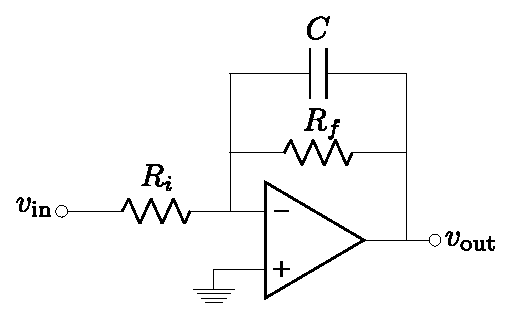
\includegraphics[width = 6.5cm]{V8_pasabajas_activo.eps}
	\end{figure}
	
	Utilizando LTspice se puede hacer la simulación de respuesta en frecuencia del circuito utilizando el modelo spice del amplificador operacional TL081 que se puede encontrar en el siguiente link:
	
	\begin{center}
		\url{http://www.ti.com/lit/zip/sloj069}
	\end{center}
	
	\begin{figure}[!ht]
		\caption{Diagrama de Bode experimental utilizando el NI ELVIS II+.}
		\label{fig:V9_elvis_pasabajas}
		\centering
		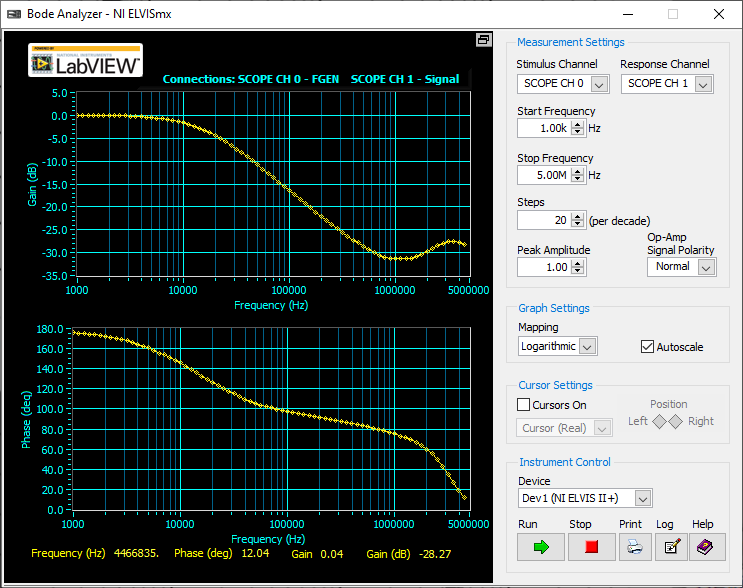
\includegraphics[width = 10cm]{V9_elvis_pasabajas.png}
	\end{figure}
	
	\begin{figure}[!ht]
		\caption{Diagramas de Bode comparativos, respuesta ideal, simulación y experimental.}
		\label{fig:V10_bodes_comparativos}
		\centering
		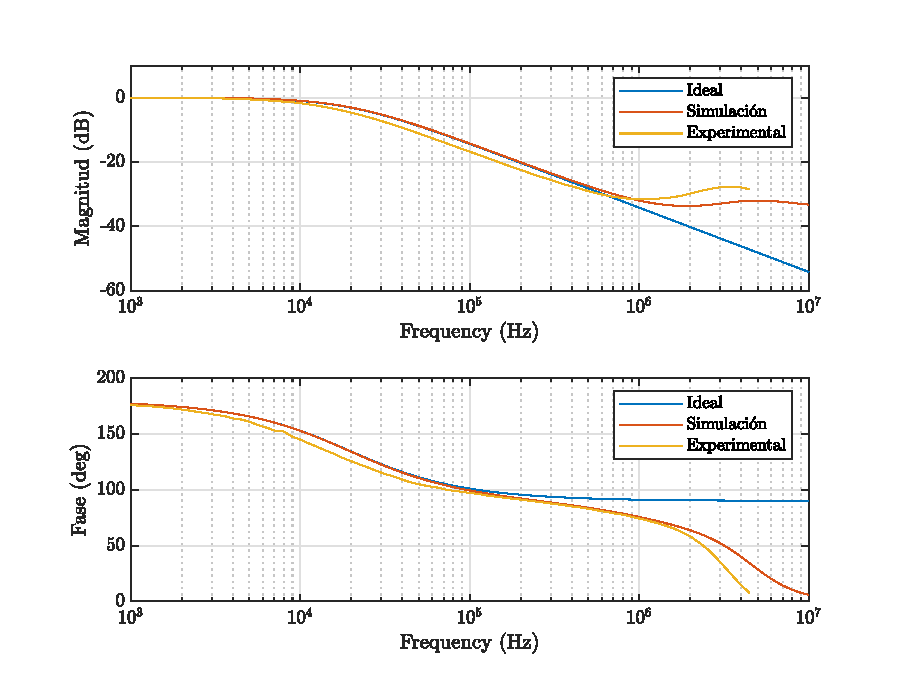
\includegraphics[width = 12cm]{V10_bodes_comparativos.eps}
	\end{figure}
	Los resultados experimentales coinciden casi a la perfección con la simulación . En frecuencias arriba de 1 MHz la respuesta se aleja del comportamiento ideal debido a las limitaciones a altas frecuencias del TL081.
	
	\section{Implementación con aproximación de primer orden}
	
		\subsection{Filtro bilineal configuración polo y cero}

		\subsection{Filtro bilineal configuración pasabajas y pasaaltas}

	
	\section{Implementación con aproximación de segundo}
	
		\subsection{Filtro bicuadrático configuración polo cero}
	\chapter{Oscilador caótico utilizando integradores de orden fraccionario}

	\section{Oscilador caótico basado en funciones no lineales saturadas (SNLF)}
	
	\section{Función deestabilizadora}
	
	\section{Variables de estado del oscilador en orden fraccionario}
	
	\section{Implementación en FPAA}
	
		\subsection{Configuración bilineal polo y cero}
	
		\subsection{Configuración bilineal suma de filtros}
	\chapter{Conclusiones}
	
	En este trabajo de tesis se analizaron tres topologías para diseñar integradores de orden fraccionario. La primera consistió en utilizar un filtro bilineal el cual al ser configurado en su forma polo y cero permitió implementar integradores con ordenes dentro del rango $[0.1, 0.81]$, ordenes superiores  no fueron posibles de implementar debido a las restricciones que presenta el hardware en cuanto a la frecuencia de reloj.
	
	La segunda consistió en combinar dos filtros, un pasabajas y un pasaaltas en una configuración de suma, esta topología permitió llegar a rangos de $[0.01, 0.93]$, no obstante presentando un poco más de error en la implementación con respecto al polo y cero. Esta topología es la más versátil debido a que el rango es mayor y su metodología de diseño es sencilla.
	
	La topología bicuadrática aunque teniendo menor error, su rango es muy pequeño bajo el esquema propuesto, de $[0.01, 0.6]$, esto lo hace poco útil en la mayoría de aplicaciones. Sin embargo es una topología que aun puede estudiarse y desarrollar diversos esquemas que pueden mejorar su rendimiento.
	
	Topologías de orden superior no son recomendables debido a que la mejora de poseen no es sustancial y seria un desperdicio de recursos.
	
	Finalmente la implementación del oscilador caótico resultó exitosa y se comprobó que es posible utilizar hardware analógico embebido para implementar sistemas de orden fraccionario además de generar reglas de diseño para futuros trabajos.

\appendix
	\chapter{Códigos}

\lstinputlisting[style = MATLAB, caption =  Función syms2tf, label = cod:syms2tf]{codigos/syms2tf.m}
	\chapter{Esquemático de QuadApex v2.0}

\begin{figure}[hbtp]
	\caption{Diagrama esquemático de QuadApex v2.0}
	\centering
	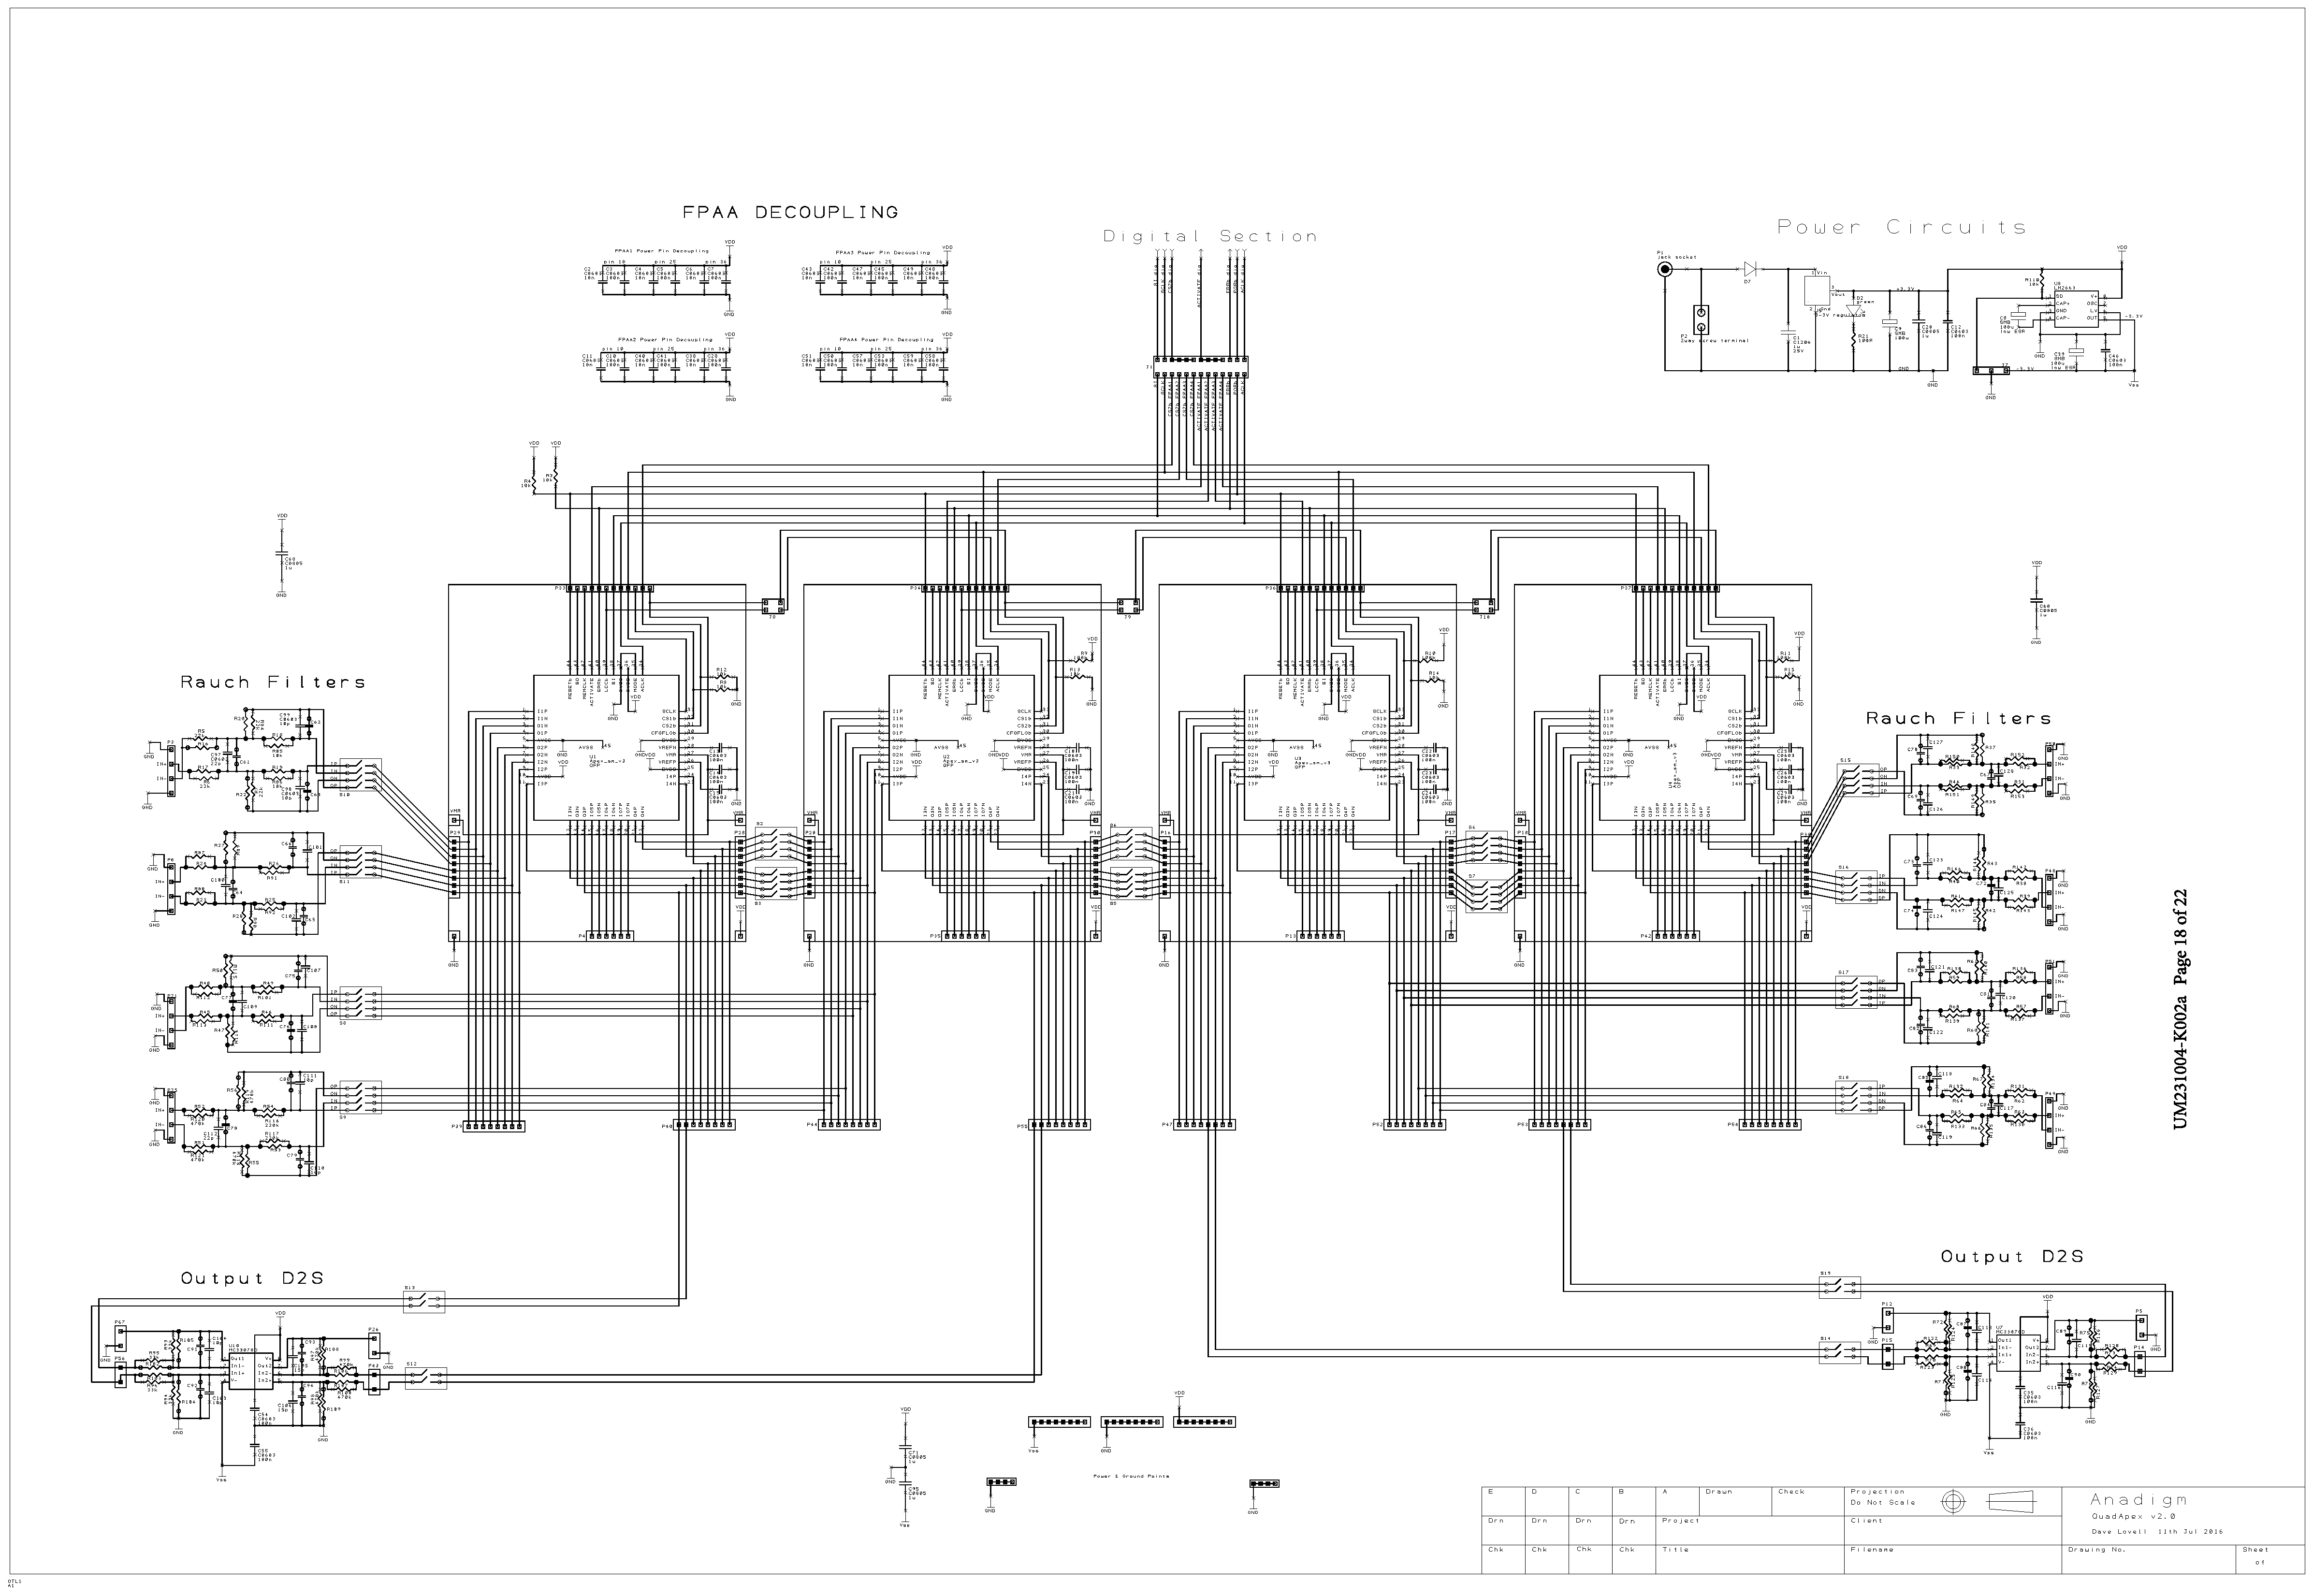
\includegraphics[width=16cm,angle=90]{Esquematico.eps}
	\label{fig:esquematico_fpaa}
\end{figure}

\backmatter

\bibliographystyle{ieeetr}
\bibliography{bibliografia}
\end{document}